\documentclass[11pt]{article}%,twocolumn
\usepackage{url}
\usepackage{cite}
\usepackage{graphicx}
\usepackage{listings}
\lstset { basicstyle=\tiny }
%\usepackage{appendix}

\begin{document}

\title{Master Thesis Preparation}
\date{\today}
\author{Dominic Bosch \\ Departement Mathematics and Computer Science \\ University of Basel}

\maketitle

\renewcommand{\abstractname}{}
\begin{abstract}
\textbf{Abstract.}
The web continously evolves into bigger complexity, allowing for ever more powerful applications. The grand challange is to retain manageable interactions between cloud applications, while applying reactivity to them. To get a hold on this, we anticipate the next change in the evolution of the web: the live web, or reactive web. By considering cloud applications as event producers and consumers we are able to apply a different level of abstraction to the web, which allows new perspectives and approaches to manifest the reactive web.
%The web over time changed its role. In the first stage, it was a passive document storage driven in client-server mode. Using web 2.0 technology in the next phase more and more desk top computer usage went into the web. Today web clouds are proliferating. We anticipate a next change in the near future: The live web or reactive web.
%The goal of this project is to enhance the web with rule-based event-condition-action (ECA) mechanisms  such that the web turns itself into an reactive entity. After an analysis of current approaches, a generalized ECA language together with a rule engine should be provided. For test and demonstration purposes, usage scenarios should be specified and new web services should be derived. As a case study, the rule engine should be integrated with the ProBinder~\cite{wwwprobinder} software, which is an advanced collaboration platform based on the shelf, binder, and register notion.
\end{abstract}


\section{Introduction}



\section{Related Work}
In ~\cite{2009-Paschke_Boley-RCER.pdf} the authors supplied general descriptions and classifications of different research efforts in terms of events, rules and reactiveness. Particularly of interest is their identification and summarization of existing research:
 \begin{itemize}
%\itemsep-1.5em
  \item Event/Action Logics, Transition Logics and Process Calculi: Events/Actions transit states and effect the lifetime of changeable properties (fluents). Used in \cite{Behrends:2008:EEA:1377798.1377801} to specify complex actions, or in to model the communication behaviour of inbound and outbound message links in rules.
  \item Dynamic/Update/Transition Logics: 
  \item Production Rule Systems:
  \item Active Databases and ECA Rule Systems:
  \item Rule-Based Complex Event Processing and Event Notification Systems: In such approaches the communication is often eased by using a middelware such as service buses. The upcoming paradigms of service-oriented architecture (SOA) and event-driven architecture (EDA) such systems allow for the reaction to the fashionable complex events. The applied reactive rules are executed to a certain context,

\end{itemize}
Language XChange uses Xcerpt(?) to express web queries. MARS was postulated in 2008 (not available?).
In contrast to standard ECA rules, which typically only have one global state, messaging reaction rules maintain a local conversation state that refelects the process exe3cution state. This supports supports the performing of different activities within process instances managed in simultaneous conversation branches.
CEP  provides enhanced situation awareness.

\subsection{Markup Languages}


\subsubsection{RuleML}
RuleML~\cite{2006-Boley-RuleML.pdf} is a rule specification standard to express both forward and backward rules for derivation, reaction, rewriting, messaging, verification and transformation. The building blocks of RuleML are predicates, derivation rules, facts, queries, integrity constraints and transformation rules.

The Rule Markup Initiative~\cite{wwwruleml}.


\subsubsection{Reaction RuleML}
Reaction RuleML~\cite{2012-Paschke_etal-ReactionRuleML.pdf} extends RuleML to allow reaction rules and complex event/action messages, e.g. for complex events processing (CEP). It adds various kinds of production, action, reaction and knowledge representation (KR) temporal/event/action logic rules, as well as (complex) event/action messages. It consists of one general reaction rule form that can be specialized, e.g. into production rules, trigger rules, ECA rules or messaging rules. Three different execution styles (active, messaging,  reasoning). Messages define inbound or outbound event messages and are used to interchange events and rule bases. A reaction rule can be globally or locally nested within other reaction or derivation rules.
RuleML Interface Description Language (RuleML IDL) is a sublanguage of Reaction RuleML and allows the description of public rule functions.


\subsubsection{JSON Rules}


\subsection{Rule Engines}

\subsubsection{Kynetic Rules Engine}
A framework presented in ~\cite{bookTheLiveWeb}

\subsubsection{Rule Responder}
Rule Responder~\cite{2007-Paschke_etal-RuleResponder.pdf} is a project to extend the Semantic Web towards a Pragmatic Web infrastructure for collaborative human-computer networks, which they call an architecture of a Pragmatic Agent Web (PAW). It supports the formation of virtual groupings and allows semi-automated agents with their individual contexts, decisions and actions. The authors postulate agents empowered with automatic rule-driven data transformation, decision derivation from existing knowledge and reaction according to changed situations or occurred events. The work done in this project concentrates on a layer on top of a rule engine and language, and thus allows for a combination of arbitrary rule-based systems via their framework. This is achieved through the usage of general messge oriented communication interfaces and a platform-independent rule interchange format.
\\
The authors of Rule Responder built their reference system on top of the Mule~\cite{wwwmuleesb} open-source Enterprise Service Bus (ESB) which acts as a communication middleware. The decision to use Mule was made because it goes beyond the typical definition of an ESB by providing a distributable object broker to manage all sorts of service components. Each agent runs its own rbitrary rule engine. For demonstartion purposes Prova and OO jDrew were used to demonstrate the rule interchange between different rule engines.
\\
An investigated use case for Rule Responder was a symposium organization as a virtual organization.

\begin{figure*}[htb]
\begin{center}
%,angle=-90
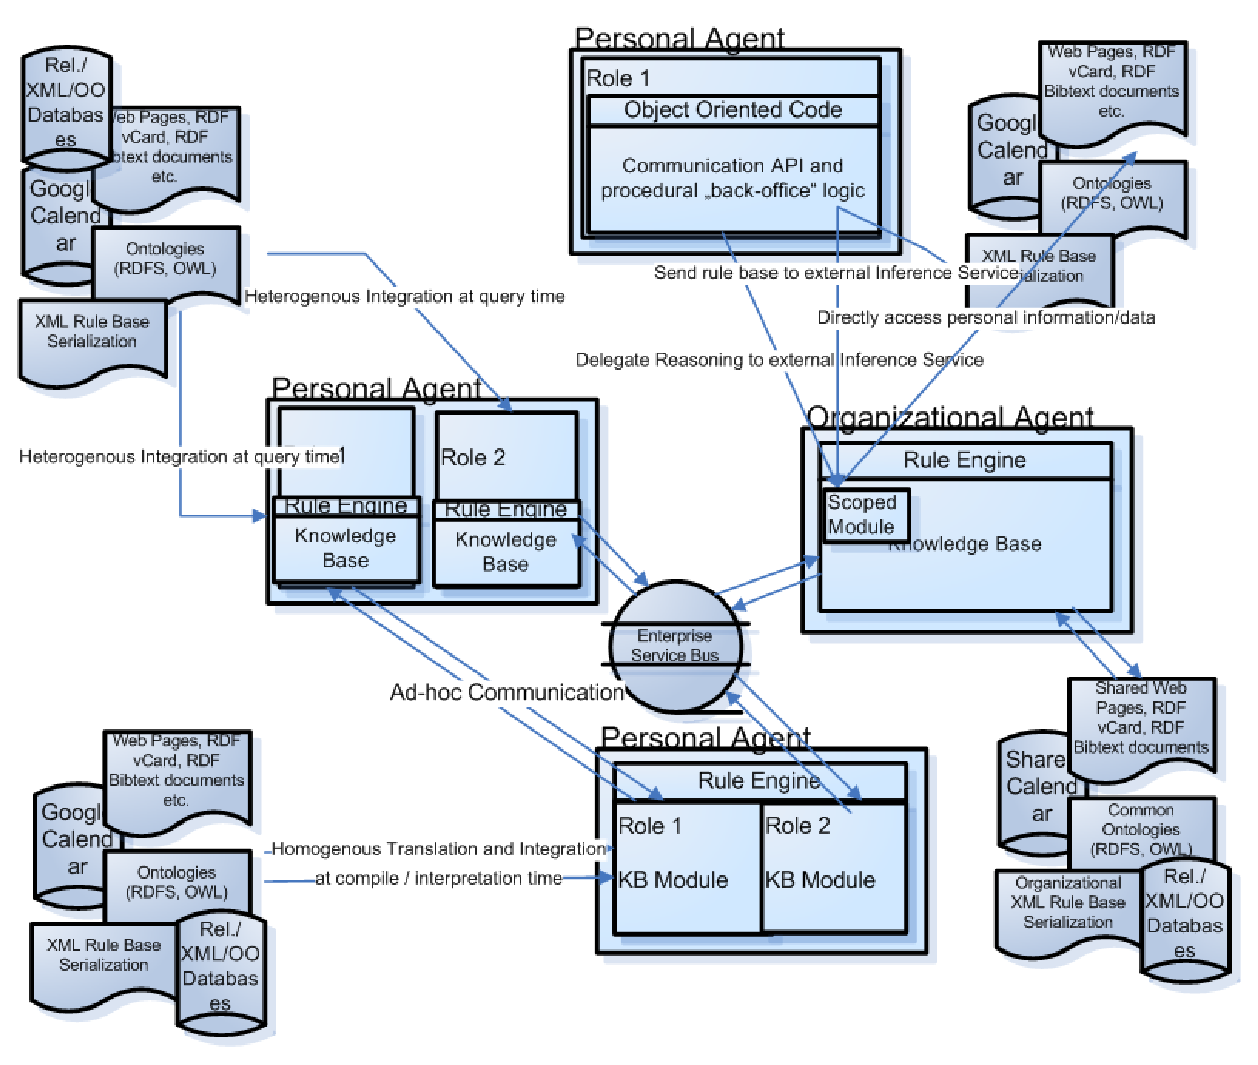
\includegraphics[scale=0.4]{img_rr01}
\caption{Rule Responder Architecture, taken from \cite{2007-Paschke_etal-RuleResponder.pdf}}
\end{center}
\end{figure*}



\subsection{Rule Languages}
\subsubsection{Kinetics Rule Language}

\subsubsection{Prova}


\subsubsection{OO jDrew}


\subsection{Towards ECA Mashups}
In \cite{2009-Pascalau_Giurca-LWAECARE.pdf}, the founders of JSON Rules~\cite{2008-Giurca_Pascalau-JSON_Rules.pdf} describe a lightweight architecture that allows to react and proact on behalf of events in the ontology of web browsers.



\section{Use Case Study}
In order to verify some of the identified related work, use cases around the succcessor of useKit~\cite{2010-Rizzotti_Burkhart-useKit.pdf} (ProBinder~\cite{wwwprobinder}) have been derived and investigated. 

\subsection{Binder Watcher}
Binder Watcher is about binders being watched and actions that are taken after certain changes to a binder. Users of ProBinder, which are involved in many different companies and project binders, tend to be confronted with a large amount of information. It is a tedious task to get the user's context back into a clean state, where the ProBinder system is ready to reflect new recent changes in an optimal way to the user. By allowing the users to identify resources (binder tabs in this case, but could also be complete binders, persons, companies, \dots) of interest, the user task can be automated to a certain extent. As soon as changes are made to the resources of interest, they are marked as read and summarized. These summaries are then provided to the user, which allows him to identify the most important changes.
\\
The Binder Watcher use case was implemented in KRL (see appendix \ref{app:uc_bw_krl}) and provided the important insight that the realization of such a use case in an ECA is a time-consuming challange. 

\subsection{Web Watcher}


\section{Conclusion}


\section{Future Work}


\bibliography{liveweb}
\bibliographystyle{related-work}

\newpage
\appendix
\renewcommand\thesection{Appendix \Alph{section}\ \ \ --}

\section{Binder Watcher KRL code} \label{app:uc_bw_krl}
\begin{lstlisting}[breaklines]
ruleset a2236x4 {
  meta {
  	name "ProBinder Flag Notification Handler"
  	description "This is a first example on how to react on ProBinder Events"
  	author "dominic.bosch"
    //ProBinder IDs:
    // userID: 10595
    // companyID: 643
    // contextID: 16694
    // followerID: 12613
    
  	logging on
  }
  
  dispatch {}
  
  global {}
  
  // Reset all entitiy variables
  rule resetAll {
    select when probinder resetall
      send_directive("Full Reset");
      fired {
        clear ent:userID;
        clear ent:companyID;
        clear ent:contextID;
        clear ent:credentials;
        clear ent:followers;
        clear ent:newContents;
        clear ent:summary;
        clear ent:temp;
      }
  }
  
  // reset the unread content data structures
  rule reset {
    select when probinder reset
      send_directive("Reset, user credentials and followers still kept");
      fired {
        clear ent:newContents;
        clear ent:summary;
        clear ent:temp;
      }
  }
  
  // The user registers himself with email and password for the ProBinder API...
  rule register_user {
    select when probinder register
      if (event:attr('userID').as("str") neq 'null'
          && event:attr('companyID').as("str") neq 'null'
          && event:attr('contextID').as("str") neq 'null'
          && event:attr('email').as("str") neq 'null'
          && event:attr('password').as("str") neq 'null') then {
        send_directive("user registered");
      }
      fired {
        set ent:userID event:attr('userID');
        set ent:companyID event:attr('companyID');
        set ent:contextID event:attr('contextID');
        set ent:credentials uri:escape(event:attr('email')) + ":" + uri:escape(event:attr('password'));
      }
  }
  
  // The user sent an event that tells us he wants to follow somebody
  rule new_user_to_follow {
    select when probinder newfollower
      pre{
        listFollowers = ent:followers || {};
        newfollower = event:attr('followerID').as("str");
        listFollowers = listFollowers.put([newfollower], "true");
      }
      if (event:attr('userID') == ent:userID
          && newfollower neq "null") then {
            send_directive("New ProBinder User added to followers");
      }
      fired{
        set ent:followers listFollowers
      }
  }
  
  // Let the KRE check ProBinder for new unread content and process it immediately
  rule check_for_unread_content {
    select when probinder check
      pre {
        r = http:get("https://" + ent:credentials + "@probinder.com/service/36/unreadcontent");
        arr = r{"content"}.decode();
      }
      send_directive("Checked ProBinder for unread content, found: " + arr.length());
      fired {
        set ent:newContents arr;
        raise explicit event processnewcontents;
      }
    
  }
  
  // Work (new unread content) from ProBinder to process
  rule process_new_contents {
    select when explicit processnewcontents
    // Process only the unread contents from people we are following,
    // filter condition omits unnecessary rules invocation
    foreach ent:newContents.filter(
      function(d) {ent:followers.pick("$."+d.pick("$.userId")) != null}
    ) setting(nc)
      pre {
        s = ent:summary || {};
        cid = nc.pick("$.id");
        r = http:get("https://" + ent:credentials
          + "@probinder.com/service/2/get?id=" + cid
          + "&service=" + nc.pick("$.serviceId"));
        arr = r{"content"}.decode();
        
        userid = arr.pick("$.userId");
        storeKey = arr.pick("$.lastModified");
        truncStr = arr.pick("$.text");//.extract(re/^.{100}/gi); // should shorten the text...
        
      //TODO Process different kind of unread contents differently
        str = {"content": truncStr}; //[0]
        s = s.put([userid, storeKey], str);
      }
      http:get("https://" + ent:credentials + "@probinder.com/service/2/setread?id=" + cid);
      always {
        set ent:summary s;
      }
    
  }
  
  rule send_summary{
    select when probinder heartbeat
    always {
      clear ent:temp;
      raise explicit event filltemp;
    }
  }
  
  rule fill_temp{
    select when explicit filltemp
    always {
      set ent:temp ent:summary;
      raise explicit event mergecontent;
    }
  }
  
  // When somebody sends a periodic heartbeat, this summary is produced
  // The periodic invocation of this rule might be possible to implement in the KRE
  rule merge_content {
    select when explicit mergecontent
    foreach ent:temp setting (userID)
      pre {
        s = ent:temp;
        userBulk = s.pick("$."+userID);
        sumry = userBulk.pick("$..content").join(" ");
      }
      http:get("https://" + ent:credentials + "@probinder.com/service/27/save?companyId="
        + ent:companyID + "&context=" + ent:contextID + "&text=test");
      send_directive("Stored summary in your predefined binder:" + sumry);

  }
  
  rule print_summary {
    select when probinder printsum
      send_directive(ent:summary);
  }
}
\end{lstlisting}

\end{document}
